\section{Application to WS$_2$ nanostructures}
\label{sec:results_sample}

Following the discussion of the vacuum results, we now move
to present the application of our method to the parametrisation
of EEL spectra recorded on samples.
%
Specifically, we will consider data taken on the WS$_2$ nanostructures
presented in~\cite{SabryaWS2} and reviewed in Sect.~\ref{sec:tmd}.
%
These nanostructures exhibit a flower-like configuration where different layers
of material combine to form the petals and the stem of the flowers.
%
Their geometrical configuration is such that depending on the region
of the nanostructure that one is imaging the spectra will be sensitive
to different thicknesses and orientations of the material.
%
The parametrisation of the ZLP for these in-sample spectra will then be used
to subtract the ZLP contribution and extract the bandgap from
the behaviour of $I_{\rm inel}(\Delta E)$ in the very low-loss region.

\paragraph{Training dataset.}
%
Fig.~\ref{fig:ws2positions} displays
low-magnification TEM images of two different regions of
the WS$_2$ nanoflowers, denoted by A and B in the following.
%
In each image we indicate with numbers the specific positions where
EEL spectra have been recorded, both in the sample and in vacuum for
reference purposes.
%
In the upper image the difference in contract is correlated to the material
thickness, with higher contrast corresponding to thinner regions.
%
Here our ZLP parametrisation strategy will be applied separately
to samples A and B, since in each case the measurements have
been obtained with different electron microscopes and
operation settings.

%%%%%%%%%%%%%%%%%%%%%%%%%%%%%%%%%%%%%%%%%%%%%%%%%%%%%%%%%%%%%%%%%%%%%%%
\begin{figure}[t]
\begin{centering}
  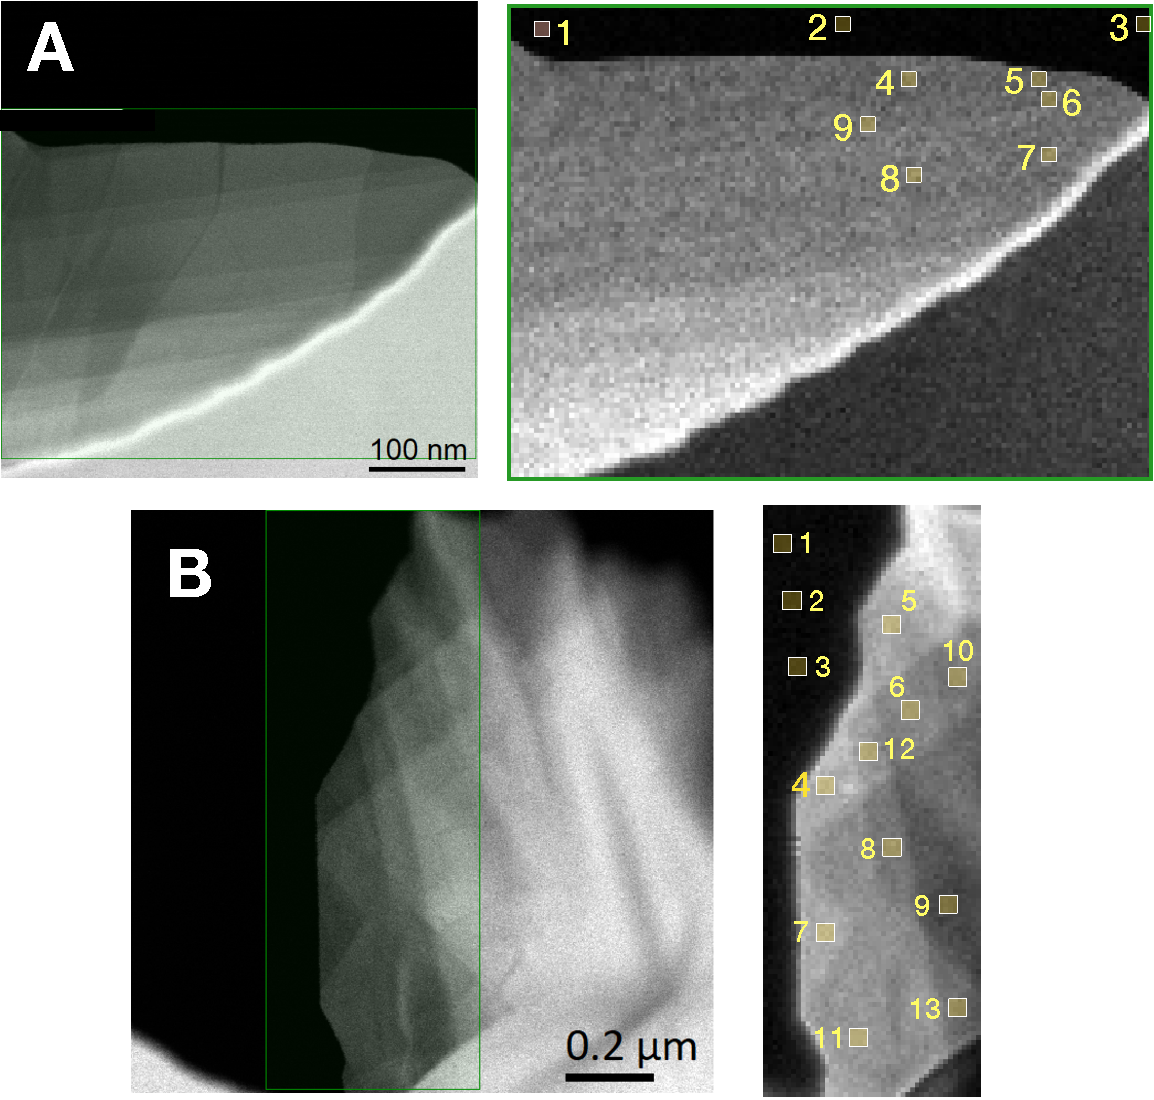
\includegraphics[width=0.87\linewidth]{plots/Spectra_location.pdf}
  \caption{Low-magnification TEM images of two different regions of
    the WS$_2$ nanoflowers, denoted by A and B in the following.
    %
    In each image we indicate with numbers the specific positions where
    EEL spectra have been recorded, both in the sample and in vacuum for
    reference purposes.
    %
    In the upper image the difference in contract is correlated to the material
    thickness, with higher contrast corresponding to thinner regions.
  }
\label{fig:ws2positions}
\end{centering}
\end{figure}
%%%%%%%%%%%%%%%%%%%%%%%%%%%%%%%%%%%%%%%%%%%%%%%%%%%%%%%%%%%%%%%%%%%%%%%%%%

In Table~\ref{table:sampledata} we collect the most relevant properties of the spectra collected
in the locations indicated in Fig.~\ref{fig:ws2positions} using the same convention as
in Table~\ref{table:sampledata}.
%
As mentioned above the A and B sets of spectra have been acquired with different microscopes and thus are
not directly comparable.
%
Then in Table~\ref{table:sampledata_summary} we display
the mean value and uncertainty of the first local minima $\Delta E_{\rm min}$
    of the spectra in sets A and B, as well as the corresponding values of the hyper-parameters
    $\Delta E_I$ and $\Delta E_{II}$ defined in Fig.~\ref{fig:EELS_toy}.
    %
    Recall that only data with $\Delta E \le \Delta E_I$ is used for the training
    of the neural network model.
    %
    We find that the location of the first minima is relatively stable
    among all the spectra belonging to given set.
    %
    For $\Delta E \ge \Delta E_{II}$ instead the training set includes only the pseudo-data
    that implements the $I_{\rm ZLP}(\Delta E)\to 0$ constraint.

%%%%%%%%%%%%%%%%%%%%%%%%%%%%%%%%%%%%%%%%%%%%%%%%%%%%%%%%%%%%%%%%%%%%%%%%%%%%%%%%%%%%%%%%%%%%%
%%%%%%%%%%%%%%%%%%%%%%%%%%%%%%%%%%%%%%%%%%%%%%%%%%%%%%%%%%%%%%%%%%%%%%%%%%%%%%%%%%%%%%%%%%%%%
\begin{table}[t]
  \begin{center}
            \renewcommand{\arraystretch}{1.50}
  \begin{tabular}{@{}ccccccccc}
\br
Set & $t_{\rm exp}$ {(}ms{)} & $E_{\rm b}$ {(}keV{)} & $N_{\rm sp}$ & $N_{\rm dat}$ & $\Delta E_{\rm min}$~(eV)  & $\Delta E_{\rm max}$~(eV)  & FWHM~(eV)  \\ 
\mr
A        &                   &                   &           &                &               &      & $\pm$         \\
B        &                   &                     &            &                &              &     & $ \pm$         \\
\br
  \end{tabular}
    \end{center}
  \caption{\small Same as Table~\ref{table:vacuumdata} now for the EEL spectra taken on WS$_2$ nanostructures.
  }
   \label{table:sampledata}
\end{table}
%%%%%%%%%%%%%%%%%%%%%%%%%%%%%%%%%%%%%%%%%%%%%%%%%%%%%%%%%%%%%%%%%%%%%%%%%%%%%%%%%%%%%%%%%%%%%%%%%5
%%%%%%%%%%%%%%%%%%%%%%%%%%%%%%%%%%%%%%%%%%%%%%%%%%%%%%%%%%%%%%%%%%%%%%%%%%%%%%%%%%%%%%%%%%%%%


%%%%%%%%%%%%%%%%%%%%%%%%%%%%%%%%%%%%%%%%%%%%%%%%%%%%%%%%%%%%%%%%%%%%%%%%%%%%%%%%%%%%%%%%%%%%%
%%%%%%%%%%%%%%%%%%%%%%%%%%%%%%%%%%%%%%%%%%%%%%%%%%%%%%%%%%%%%%%%%%%%%%%%%%%%%%%%%%%%%%%%%%%%%
\begin{table}[t]
  \begin{center}
            \renewcommand{\arraystretch}{1.50}
  \begin{tabular}{@{}ccccccccc}
\br
Set & $\Delta E_{\rm min}$~(eV)  &  $\Delta E_I$~(eV)  &  $\Delta E_{II}$~(eV)   \\
\mr
A        &    $\pm$                &                   &              \\
B        &    $\pm$               &                     &               \\
\br
  \end{tabular}
    \end{center}
  \caption{\small The mean value and uncertainty of the first local minima, $\Delta E_{\rm min}$
    of the spectra in sets A and B as well as the corresponding values of the hyper-parameters
    $\Delta E_I$ and $\Delta E_{II}$ defined in Fig.~\ref{fig:EELS_toy}.
    %
    Recall that only EELS data with $\Delta E \le \Delta E_I$ is included in the training dataset.
  }
   \label{table:sampledata_summary}
\end{table}
%%%%%%%%%%%%%%%%%%%%%%%%%%%%%%%%%%%%%%%%%%%%%%%%%%%%%%%%%%%%%%%%%%%%%%%%%%%%%%%%%%%%%%%%%%%%%%%%%5
%%%%%%%%%%%%%%%%%%%%%%%%%%%%%%%%%%%%%%%%%%%%%%%%%%%%%%%%%%%%%%%%%%%%%%%%%%%%%%%%%%%%%%%%%%%%%


%
A collection of electron loss spectra acquired at different positions 
at the specimen is used to construct the neural network training inputs. 
%
These sets of data were obtained directly from~\cite{SabryaWS2}.
%
A specimen image of the positions can be observed in figure~\ref{fig:ws2positions}.  
This nanostructure exhibits flat layers with different thicknesses, which 
can be distinguished from the picture as color differences.
%
Energy loss spectra obtained at positions 1-3 are vacuum recordings, 
positions 4-13 represent in-sample data.
%
One layer (S-W-S) WS$_2$ has a thickness of around 0.9 nm. 
The thickness of the specimen at location 5 is 2.11 nm ($\sim$2 layers).
%
\begin{figure}[ht]
\begin{centering}
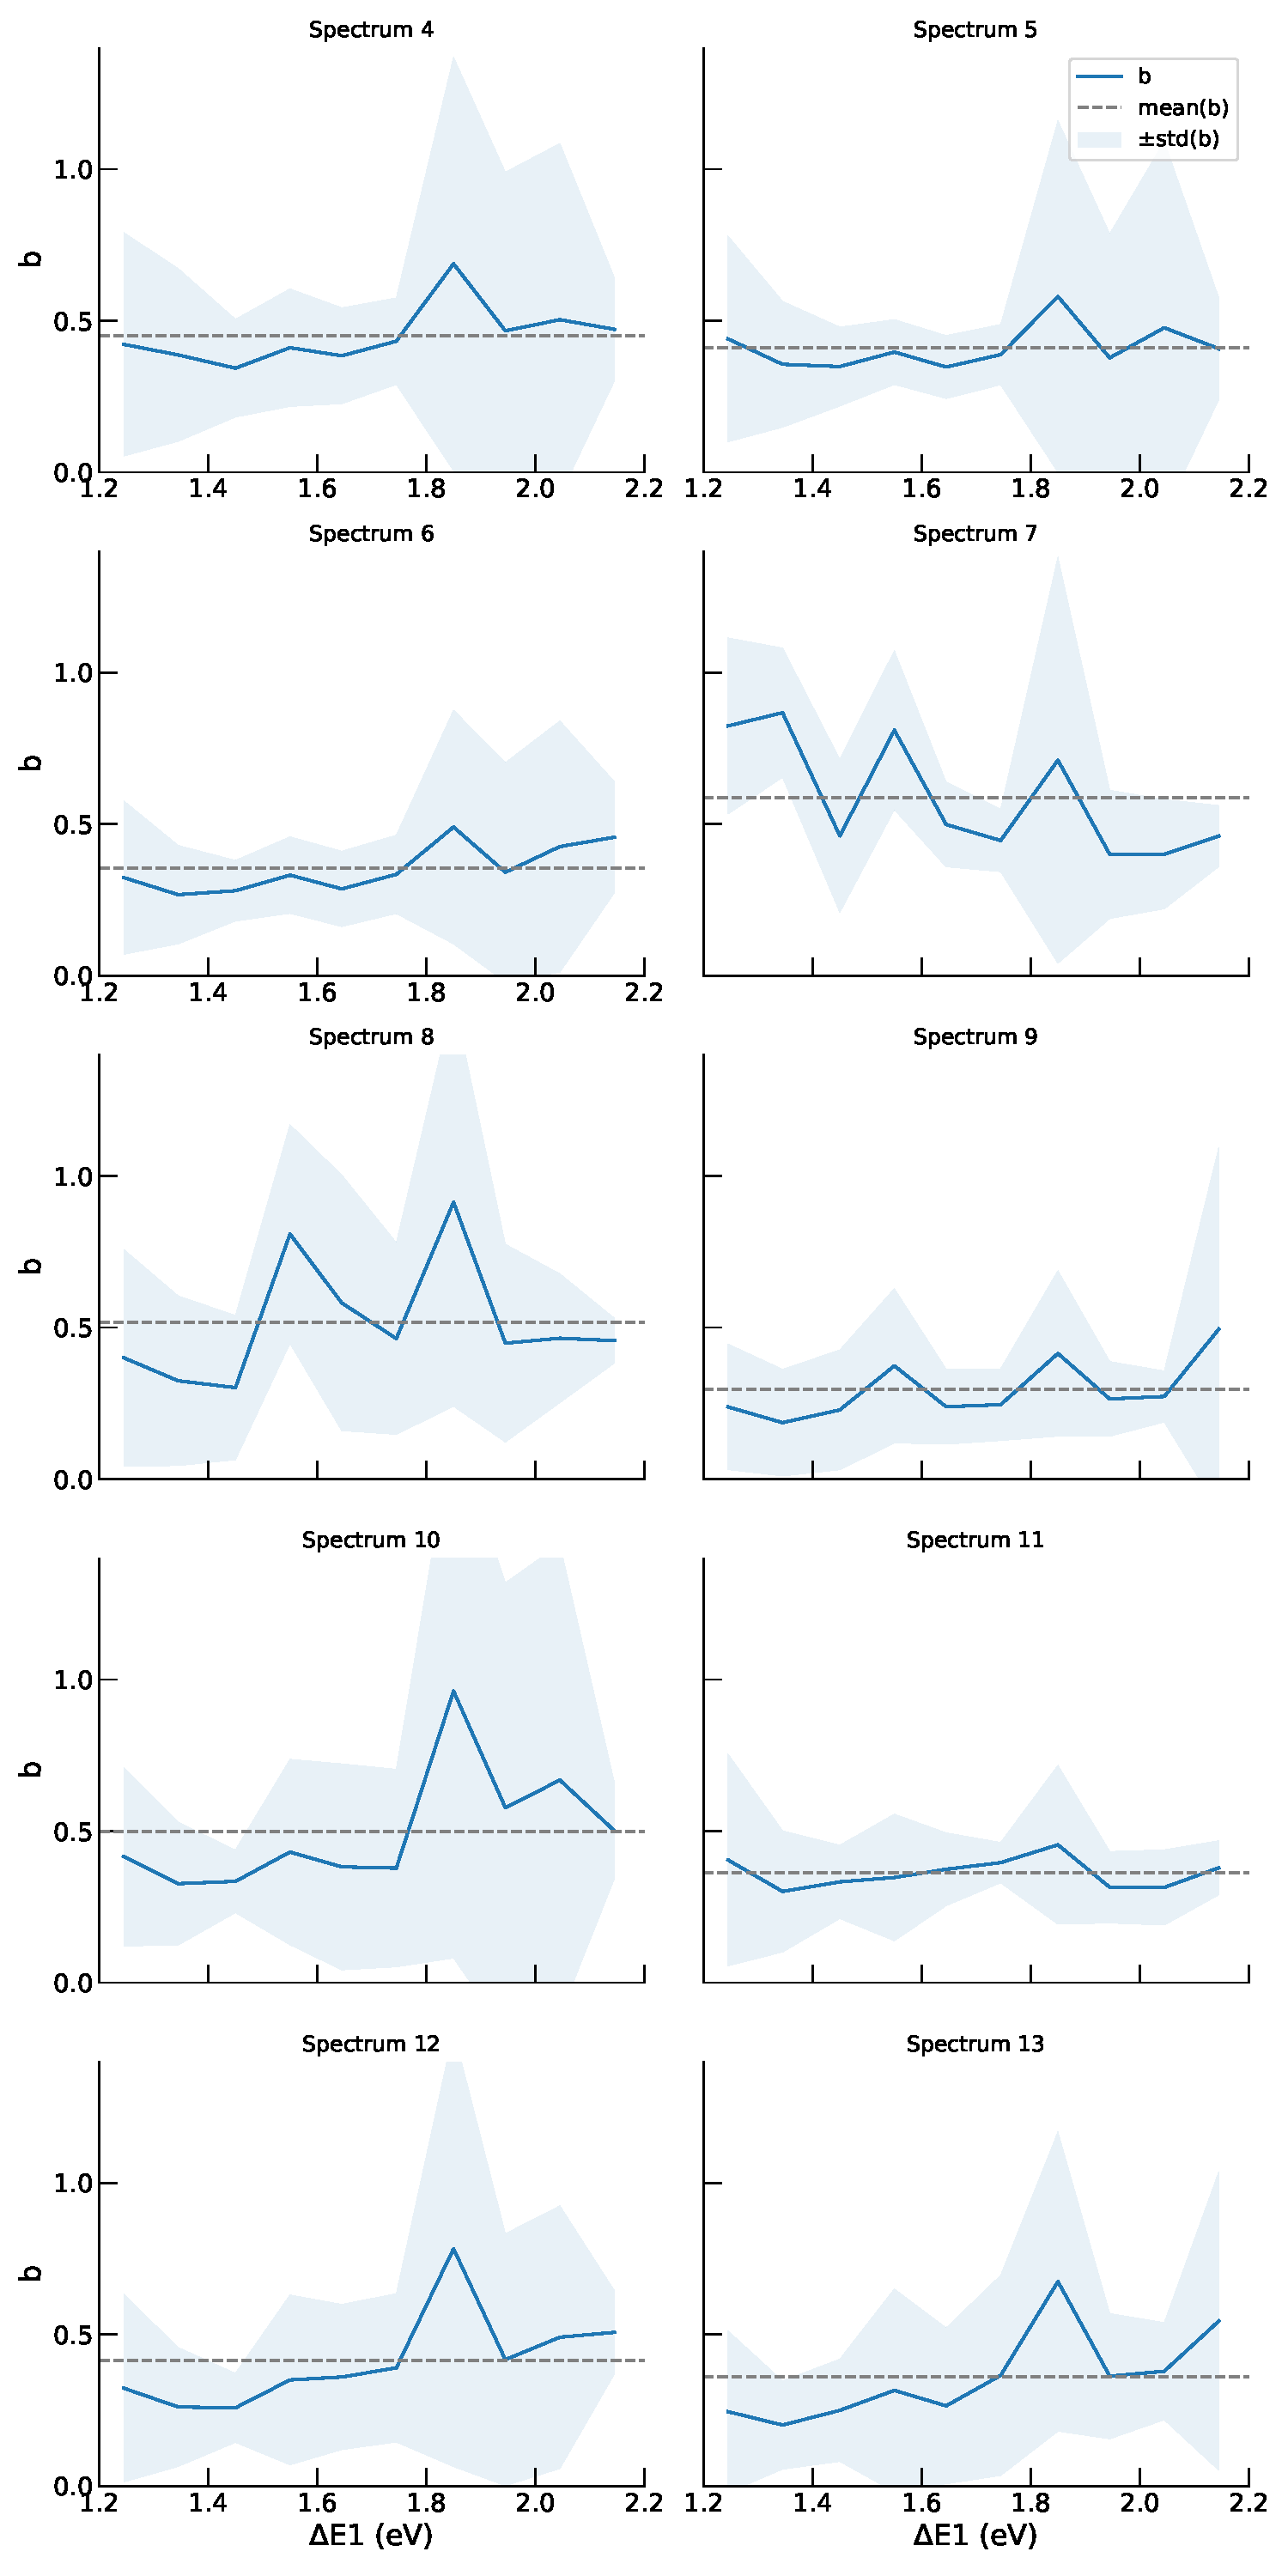
\includegraphics[width=0.6\linewidth]{plots/bvalues.pdf} 
\caption{Values for b at different positions}
\label{fig:bvalues}
\end{centering}
\end{figure}

\begin{figure}[ht]
\begin{centering}
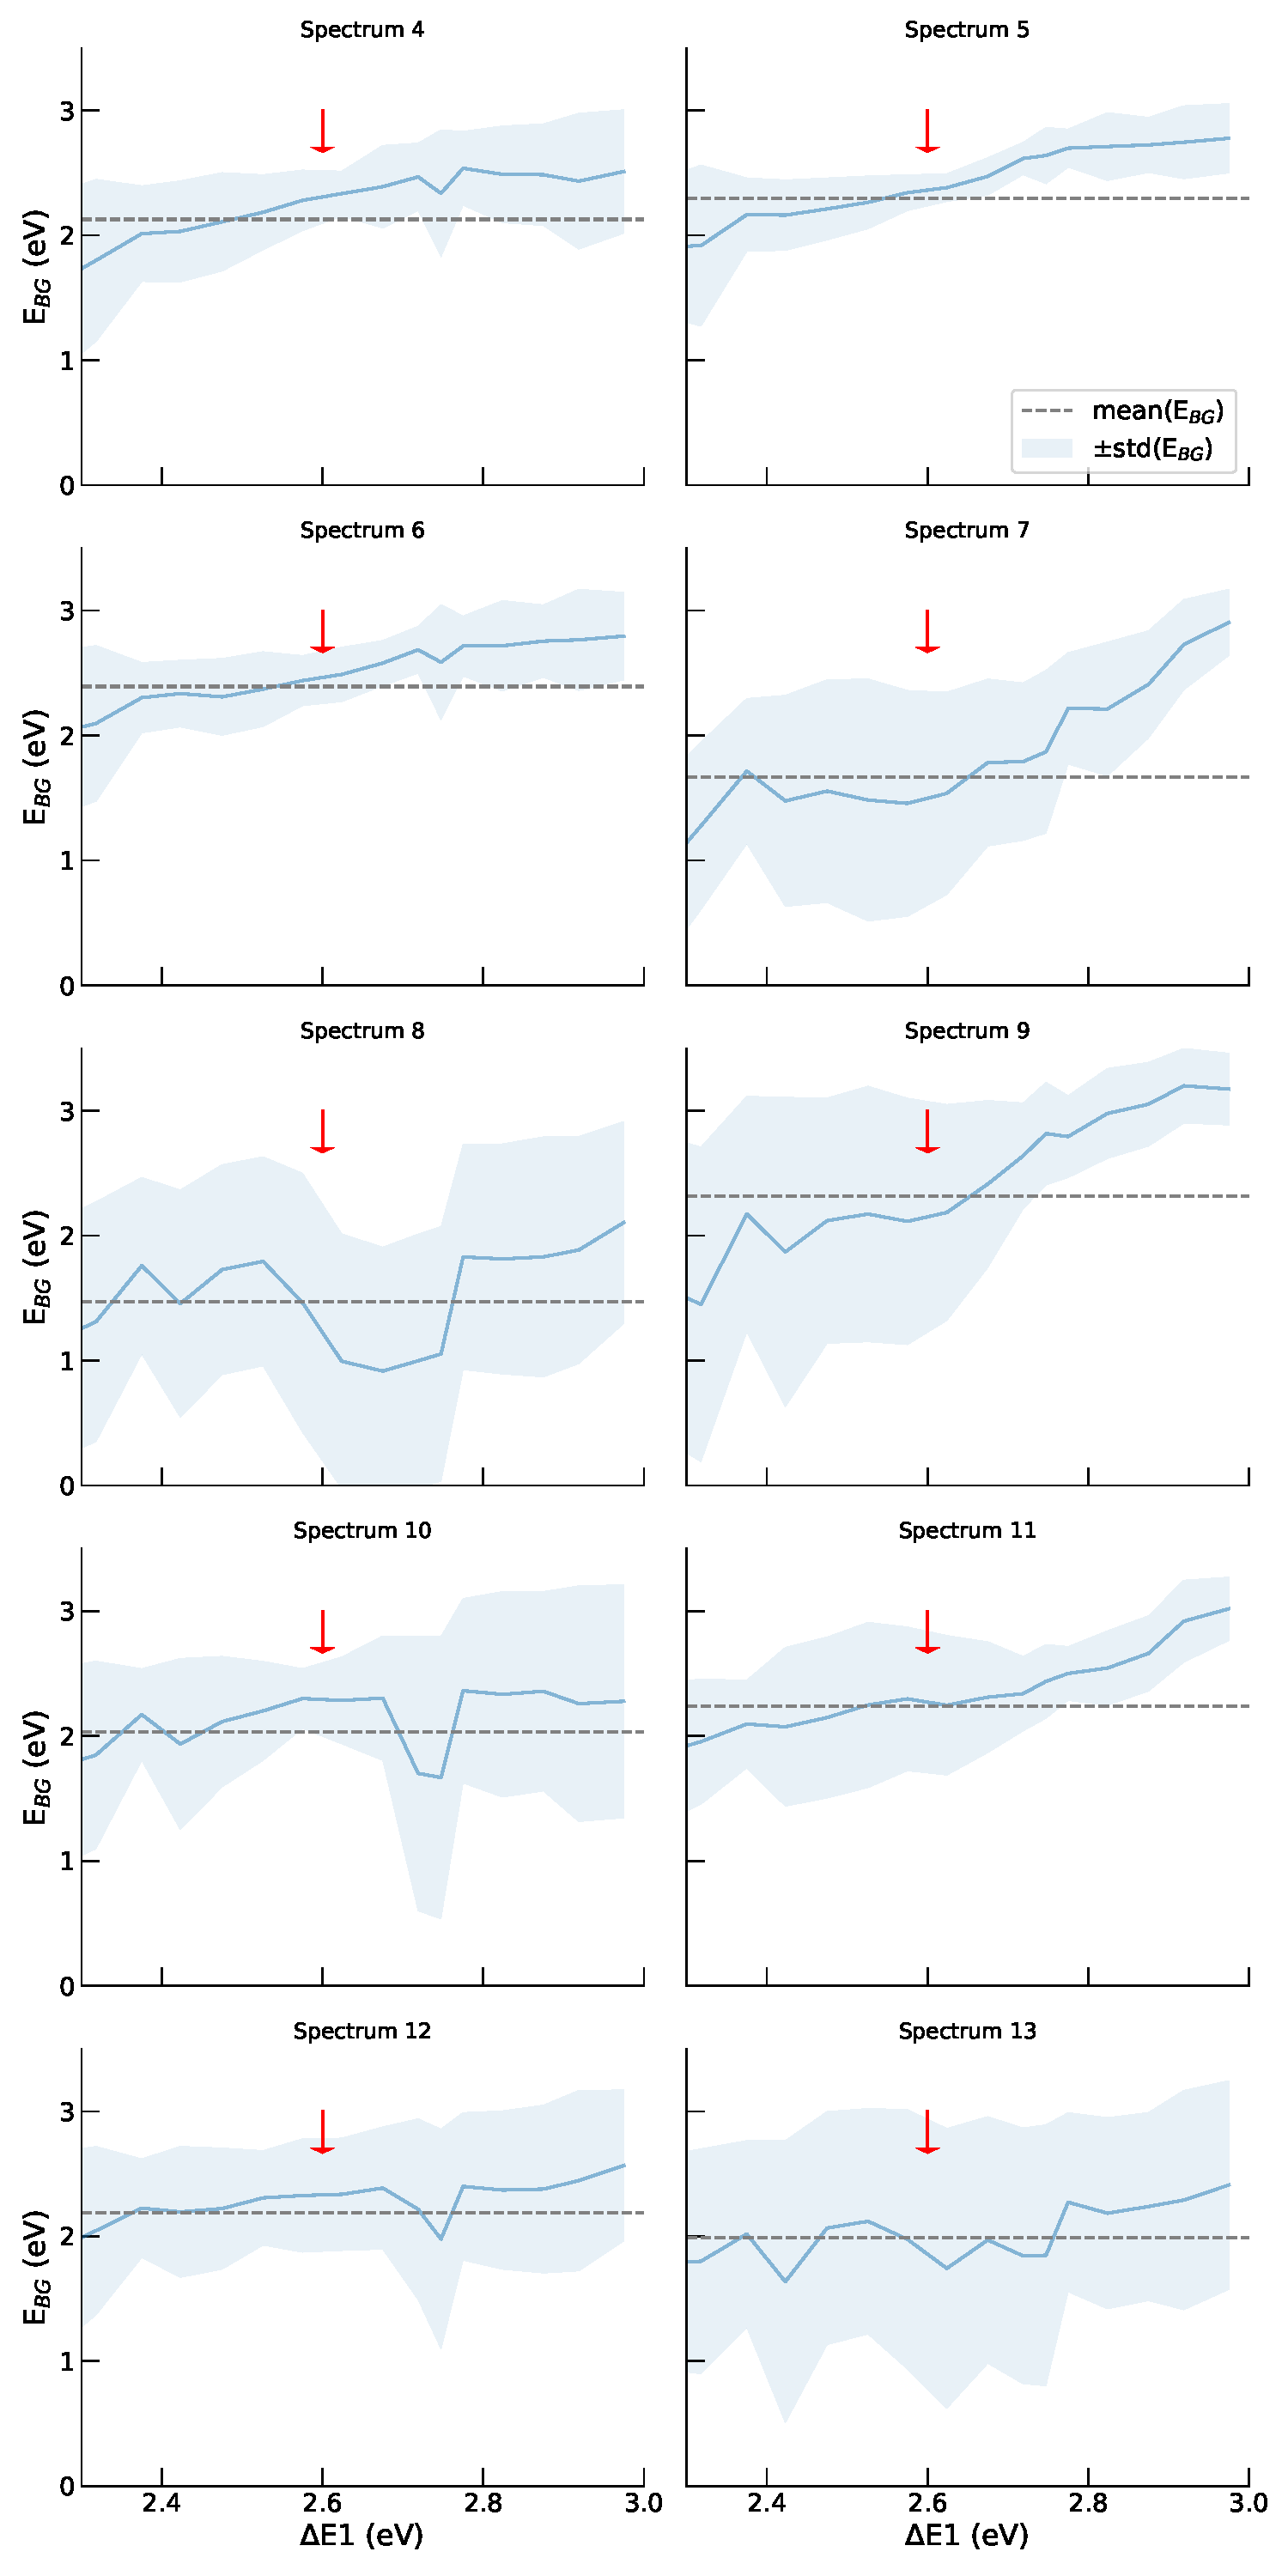
\includegraphics[width=0.6\linewidth]{plots/bgvalues.pdf} 
\caption{Values for E$_{BG}$ at different positions}
\label{fig:bvalues}
\end{centering}
\end{figure}




\subsection{Band-gap determination}


For each replica, the predicted ZLP is subtracted from the individual 
experimental spectra to obtain one set of subtractions. 
Repeating this procedure yields a collection of $N_{rep}$ subtractions 
for each original spectrum, over which statistical properties such as 
median and variance can be calculated.\newline
%
From these subtractions, which contain the 'pure' sample data, 
it is possible estimate the band gap. To a first approximation,
this can be done as the inflection point of the rising intensity.
%
The value can also be roughly estimated from the onset of the absorption 
or from a linear fit to the maximum positive slope in the 
EELS spectrum~\cite{Schamm:2003}. 
%
However, a more accurate and reliable determination is based on the work of 
Rafferty and Brown~\cite{Rafferty:2000}. The onset of the subtracted spectrum 
for a a material with a direct bandgap is expected to follow a function of the type
\begin{equation}\label{eq:I1}
    I(E) = I_0 + c\cdot(dE-E_{BG})^{(b)}
\end{equation}
where I$_0$ and c are constants, b equals 0.5, $\Delta$E is the energy loss and E$_{BG}$ 
is the bandgap energy.For an indirect bandgap, the power of $(1/2)$ changes to $(3/2)$. 
%
Therefore, the bandgap nature (direct or indirect) can be extracted by 
least-squares fitting of each k-th replica subtracted spectrum to equation~\ref{eq:I1}.
%
By averaging over all replicas, one can determine $\textless{b}\textgreater{}$, 
$\textless{E_{BG}}\textgreater{}$ 
and their uncertainties, while keeping track of how the free parameter
E$_{BG}$ is sensitive to the choice of $\Delta$E$_1$, which marks the onset
of the subtracted spectrum intensity.
%

